% =============================================================================
% MutualFundMarketing_slides.tex
% Conference: Dishui Lake Finance Conference International (DFCI) 2026
% Length: 30 minutes
% Compile with: pdflatex MutualFundMarketing_slides.tex (twice)
% =============================================================================
\documentclass[11pt, aspectratio=169]{beamer}

\usepackage{helvet}
\usepackage[default]{lato}
\usepackage{array}
\usepackage{colortbl}
\usepackage{latexsym,xcolor}
\usepackage{tikz}
\usetikzlibrary{positioning,calc,arrows,shapes.misc,matrix,shapes,arrows,fit,tikzmark}
\usepackage{amsmath}
\usepackage{mathpazo}
\usepackage{hyperref}
\usepackage{graphicx}
\usepackage[space]{grffile}
\usepackage{multirow}
\usepackage{booktabs}
\usepackage{changepage}
\usepackage{appendixnumberbeamer}

% -----------------------------------------------------------------------
% Colors
% -----------------------------------------------------------------------
\definecolor{myblue}{RGB}{0,114,178}
\definecolor{mygold}{RGB}{185,151,91}
\definecolor{myred}{RGB}{213,94,0}
\definecolor{mygreen}{RGB}{0,158,115}
\definecolor{MyBackground}{RGB}{255,253,218}

\hypersetup{colorlinks=false, linkbordercolor={white}, linkcolor={myblue}}

% -----------------------------------------------------------------------
% Beamer appearance
% -----------------------------------------------------------------------
\setbeamercolor{frametitle}{fg=myblue}
\setbeamercolor{title}{fg=black}
\setbeamercolor{itemize item}{fg=myblue}
\setbeamercolor{itemize subitem}{fg=myblue}
\setbeamercolor{enumerate item}{fg=myblue}
\setbeamercolor{enumerate subitem}{fg=myblue}
\setbeamercolor{button}{bg=MyBackground,fg=myblue}
\setbeamercolor{block title}{fg=white, bg=myblue}
\setbeamercolor{block body}{bg=myblue!8!white}
\setbeamercolor{block title alerted}{fg=white, bg=mygold!80!black}
\setbeamercolor{block body alerted}{bg=mygold!12!white}
\setbeamertemplate{footline}[frame number]
\setbeamertemplate{navigation symbols}{}
\setbeamertemplate{itemize items}{--}
\setbeamersize{text margin left=1em,text margin right=1em}
\setbeamercolor{section in toc}{fg=myblue}

% -----------------------------------------------------------------------
% Environments and macros
% -----------------------------------------------------------------------
\newenvironment{wideitemize}{\itemize\addtolength{\itemsep}{6pt}}{\enditemize}

\newcommand{\hl}[1]{\textcolor{myblue}{\textbf{#1}}}
\newcommand{\hlg}[1]{\textcolor{mygold}{\textbf{#1}}}
\newcommand{\muted}[1]{\textcolor{gray}{#1}}
\newcommand{\good}[1]{\textcolor{mygreen}{#1}}
\newcommand{\bad}[1]{\textcolor{myred}{#1}}

% -----------------------------------------------------------------------
% Title metadata
% -----------------------------------------------------------------------
\title[]{\texorpdfstring{%
  \vspace*{-2ex}\textcolor{myblue}{The Zero-Sum Game of Mutual Fund Marketing}%
}{The Zero-Sum Game of Mutual Fund Marketing}}

\author[]{}

\institute[]{
  \small
  \begin{tabular}{cccc}
    Haiwei Chen & Ilias Filippou & Jeong Ho (John) Kim & \textbf{Jiangyuan Li} \\
    SUFE & FSU & FSU & SUFE \\
  \end{tabular}
}

\date{Dishui Lake Finance Conference International \\ May 2026}

% =============================================================================
\begin{document}
% =============================================================================

\begin{frame}
  \maketitle
\end{frame}

\begin{frame}{Outline}
  \tableofcontents
\end{frame}

% =============================================================================
\section{Motivation}
% =============================================================================

\begin{frame}{Mutual Fund Marketing: What We Know}

\begin{wideitemize}
  \item Asset management has grown dramatically — AUM and fund counts have
  surged worldwide; \hl{investor search costs} are a first-order friction in
  capital allocation (Hortaçsu \& Syverson, 2004; Huang, Wei \& Yan, 2007)

  \item U.S.\ mutual funds spend roughly \hl{one-third of fee revenue on marketing};
  advertising, broker distribution, and platform visibility drive significant
  fund-level inflows (Sirri \& Tufano, 1998; Gallaher, Kaniel \& Starks, 2008)

  \item A growing literature studies \hl{social media marketing} of funds:
  De Haan et al.\ (2025), Kacperczyk \& Pagnotta (2026), and Li et al.\ (2026)
  examine mutual fund livestreaming on retail platforms in China
\end{wideitemize}

\vspace{0.3cm}
\begin{block}{An open question}
  Most prior work evaluates marketing at the \textbf{fund level}, even though
  decisions are made and success should be judged at the \textbf{family level}.
  Does fund-level marketing translate into family-level growth?
\end{block}

\end{frame}

% -----------------------------------------------------------------------

\begin{frame}{This Paper}

\begin{wideitemize}
  \item We study \hl{social media livestreaming} as a marketing tool used by
  Chinese mutual fund families on the Tiantian Fund platform, 2020--2025

  \item We evaluate marketing effects at both the \textbf{fund level} and the
  \textbf{family level}, using 25,685 livestreaming events across 180 families

  \item We analyze \textbf{795 transcripts} with a large language model to
  understand what communication strategies attract outside capital
\end{wideitemize}

\vspace{0.3cm}
\textbf{Main findings:}
\begin{enumerate}
  \item Livestreaming generates \hl{zero} family-level flows or revenue change ---
  it reallocates capital within families, not across them

  \item Families use livestreams as an \hl{internal open market operation}: steering
  investors from overcapitalized to undercapitalized funds

  \item Market competition creates a \hl{prisoner's dilemma}: families must
  livestream to defend existing assets, not to attract new ones

  \item Only \hl{``hard information''} (past performance, social proof) distinguishes
  families that successfully attract outside capital
\end{enumerate}

\end{frame}

% =============================================================================
\section{Institutional Background}
% =============================================================================

\begin{frame}{China's Mutual Fund Market}

\begin{columns}[T]
\begin{column}{0.52\textwidth}
\textbf{A large and rapidly growing market:}
\begin{itemize}
  \item Publicly offered fund AUM grew from CNY 8.4 trillion (2015) to
  over CNY 31 trillion by 2024
  \item Our sample covers \hl{5,809} actively managed equity/hybrid funds
  across \hl{180} fund families
  \item Third-party platforms (Alipay, JD Finance, Tiantian) distribute
  the majority of retail fund purchases
\end{itemize}

\vspace{0.25cm}
\textbf{Retail-dominated investor base:}
\begin{itemize}
  \item Retail investors account for the bulk of fund flows
  \item Strong \hl{flow-performance sensitivity} — investors chase
  recent winners (Sirri \& Tufano, 1998)
  \item High turnover: investors redeem quickly after underperformance
\end{itemize}
\end{column}
\begin{column}{0.46\textwidth}
\textbf{Why marketing matters here:}
\begin{itemize}
  \item With thousands of funds across hundreds of families, \hl{search
  costs} are severe for retail investors
  \item Fund families compete intensively for investor \hl{attention},
  particularly on third-party platforms where all families coexist
  \item Marketing is a primary lever for distinguishing one family's
  products from another's
\end{itemize}

\vspace{0.25cm}
\textbf{Our setting (Tiantian Fund):}
\begin{itemize}
  \item One of China's top three retail fund platforms
  \item Hosts livestream channels for all major fund families
  \item Provides shopping cart purchase integration
\end{itemize}
\end{column}
\end{columns}

\end{frame}

% -----------------------------------------------------------------------

\begin{frame}{The Rise of Livestream Marketing}

\begin{columns}[T]
\begin{column}{0.55\textwidth}
\textbf{How it began (2020):}
\begin{itemize}
  \item COVID-19 disrupted traditional sales channels:
  in-branch consultations, roadshows, and fund fairs were suspended
  \item Fund families pivoted to \hl{real-time video broadcasts} on
  retail platforms to reach investors directly
  \item By 2021, every major fund family operated its own livestream channel
\end{itemize}

\vspace{0.2cm}
\textbf{Regulatory framework (AMAC, 2021):}
\begin{itemize}
  \item Asset Management Association of China formalized
  guidance on livestream marketing
  \item Requirements: investor education, product disclosure,
  compliance pre-approval, and risk warnings
  \item \hl{Compliance approval is obtained days in advance}:
  topic and featured funds are pre-planned, not spontaneous
\end{itemize}
\end{column}
\begin{column}{0.43\textwidth}
\textbf{Scale of the phenomenon:}
\begin{itemize}
  \item \hl{25,685} livestreaming events in our sample
  \item July 2020 -- June 2025
  \item Families broadcast \hl{multiple times per month}
  \item Typical broadcast: 1--2 hours
  \item Live audience: hundreds to tens of thousands of viewers
\end{itemize}

\vspace{0.25cm}
\textbf{Key institutional feature:}
\begin{itemize}
  \item Families select \hl{fewer than 4 funds} per broadcast
  from their portfolio of $25+$ products
  \item This creates sharp within-family variation in
  promotional intensity --- ideal for identification
\end{itemize}
\end{column}
\end{columns}

\end{frame}

% -----------------------------------------------------------------------

\begin{frame}{How a Livestream Works}

\begin{columns}[T]
\begin{column}{0.50\textwidth}
\textbf{During the broadcast:}
\begin{itemize}
  \item A \hl{fund manager or professional host} presents to live viewers
  \item Covers market outlook and highlights 1--4 featured funds
  \item \hl{Danmaku}: real-time viewer comments scroll across the screen,
  creating interactive dialogue
  \item Risk disclosure banners appear per regulatory requirements
\end{itemize}

\vspace{0.2cm}
\textbf{The shopping cart (``Product Basket''):}
\begin{itemize}
  \item Icon in the broadcast interface expands to show featured funds
  \item Displays: fund name, asset class, risk rating,
  past performance, subscription window
  \item Viewers tap \hl{``Subscribe''} to purchase directly, without
  leaving the livestream
\end{itemize}
\end{column}
\begin{column}{0.48\textwidth}
\textbf{Treatment definition:}

\medskip
A fund is \hl{``featured''} in a quarter if any of its share classes
appears in the shopping cart during any broadcast that quarter.

\medskip
A fund is \hl{``non-featured''} if its family broadcasts that quarter
but the fund itself is not in the cart.

\vspace{0.3cm}
\begin{alertblock}{Identification}
  Within the same family and the same quarter, some funds are featured
  while others are not --- giving us a clean within-family comparison.
\end{alertblock}
\end{column}
\end{columns}

\end{frame}

% -----------------------------------------------------------------------

\begin{frame}{The Tiantian Platform: Interface Walkthrough}

\begin{columns}[T]
\begin{column}{0.31\textwidth}
  \centering
  \textbf{\small (1) Platform Portal}\\[4pt]
  
\includegraphics[width=\textwidth]{pictures/tiantian_portal.jpg}\\[5pt]
  {\footnotesize\muted{Search interface, featured livestreams, themed series, and broadcast schedule}}
\end{column}
\begin{column}{0.31\textwidth}
  \centering
  \textbf{\small (2) Livestream Room}\\[4pt]
  
\includegraphics[width=\textwidth]{pictures/tiantian_livestream.jpg}\\[5pt]
  {\footnotesize\muted{Host video, danmaku feed, risk disclosure banners, product basket icon}}
\end{column}
\begin{column}{0.31\textwidth}
  \centering
  \textbf{\small (3) Shopping Cart}\\[4pt]
  
\includegraphics[width=\textwidth]{pictures/tiantian_products.jpg}\\[5pt]
  {\footnotesize\muted{Fund name, risk level, past return, subscription window, one-click purchase}}
\end{column}
\end{columns}

\vspace{0.2cm}
\muted{\small Screenshots from Tiantian Fund (天天基金), one of China's leading third-party fund distribution platforms. All broadcasts go through the same portal, giving us a uniform cross-family observation window.}

\end{frame}

% =============================================================================
\section{Data and Empirical Design}
% =============================================================================

\begin{frame}{Sample and Key Variables}

\begin{columns}[T]
\begin{column}{0.48\textwidth}
\textbf{Livestream data:}
\begin{itemize}
  \item \hl{25,685} events, July 2020 -- June 2025
  \item Source: Tiantian Fund platform
\end{itemize}

\vspace{0.2cm}
\textbf{Fund universe:}
\begin{itemize}
  \item \hl{5,809} actively managed equity/hybrid funds
  \item \hl{180} fund families
  \item \hl{90,850} fund-quarter observations
  \item Exclude: index, closed-end, QDII, umbrella funds
\end{itemize}

\vspace{0.2cm}
\textbf{Descriptive highlights:}
\begin{itemize}
  \item Mean fund flow: 0.38\%, SD: 42\%
  \item \hl{14\%} of fund-quarters are featured
  \item Featured funds outperform siblings in months before event
\end{itemize}
\end{column}
\begin{column}{0.50\textwidth}
\textbf{Fund flow} (return-adjusted):
\[
\text{Flow}_{i,q} = \frac{\text{TNA}_{i,q} - \text{TNA}_{i,q-1}(1+r_{i,q})}{\text{TNA}_{i,q-1}}
\]

\textbf{Family flow} (AUM-weighted aggregate):
\[
\text{FamilyFlow}_{f,q} = \frac{\displaystyle\sum_{i \in f}\!\Delta\text{TNA}_{i,q}^{\text{adj}}}{\displaystyle\sum_{i \in f} \text{TNA}_{i,q-1}}
\]

\vspace{0.15cm}
\muted{\small $\Delta\text{TNA}_{i,q}^{\text{adj}} = \text{TNA}_{i,q} - \text{TNA}_{i,q-1}(1+r_{i,q})$}

\vspace{0.25cm}
\textbf{Treatment indicators:}
\begin{itemize}
  \item \textit{Fund Livestream}: fund $i$ featured in quarter $q$
  \item \textit{Family Livestream (Oth)}: family livestreams\\
  other funds but not fund $i$
\end{itemize}
\end{column}
\end{columns}

\end{frame}

% -----------------------------------------------------------------------

\begin{frame}{Empirical Design}

\textbf{Family-level} --- does the family grow?
\[
\text{FamilyFlow}_{f,q} = \alpha_f + \delta_q
  + \beta_1\,\text{Livestream}_{f,q}
  + \mathbf{X}'_{f,q-1}\Gamma + \varepsilon_{f,q}
\]

\smallskip
\textbf{Fund-level} --- who gains, who loses?
\[
\text{FundFlow}_{i,q} = \alpha_i + \delta_q
  + \beta_1\underbrace{\vphantom{X}\text{FundLivestream}_{i,q}}_{\text{fund $i$ featured}}
  + \beta_2\underbrace{\vphantom{X}\text{FamilyLivestream(Oth)}_{i,q}}_{\text{sibling featured}}
  + \mathbf{X}'_{i,q-1}\Gamma + \varepsilon_{i,q}
\]

\vspace{0.2cm}
\begin{columns}[T]
\begin{column}{0.47\textwidth}
\textbf{Fixed effects:}
\begin{itemize}
  \item Fund / family FE absorb time-invariant unobservables
  \item Year-quarter FE control for aggregate market conditions
  \item SE clustered at the family level
\end{itemize}
\end{column}
\begin{column}{0.50\textwidth}
\textbf{Robustness:}
\begin{itemize}
  \item Family $\times$ quarter FE: absorbs all time-varying
  family shocks; identifies within-family, within-quarter
  differential
\end{itemize}
\end{column}
\end{columns}

\end{frame}

% =============================================================================
\section{Results}
% =============================================================================

\begin{frame}{Family-Level Flows: Null Across All Specifications}

\begin{columns}[T]
\begin{column}{0.56\textwidth}

\small
\textbf{Eight family-level TWFE specifications:}

\vspace{0.15cm}
\resizebox{\columnwidth}{!}{%
\begin{tabular}{lcc}
  \toprule
  Variable & Coef. & (SE) \\
  \midrule
  Family First Livestream &  3.77 & (5.12) \\
  Family Post Livestream  & $-$0.66 & (2.34) \\
  Family Livestream       &  0.90 & (2.17) \\
  Family Market Share     & $-$15.67 & (18.43) \\
  Market Livestream (Oth) & $-$0.90 & (1.65) \\
  Family Livestream Count & $-$0.09 & (0.50) \\
  \bottomrule
  \multicolumn{3}{l}{\muted{Family FE, quarter FE, controls. None significant.}}
\end{tabular}}

\end{column}
\begin{column}{0.42\textwidth}

\begin{block}{Our finding}
  Livestreaming generates \hl{zero} change in family-level flows.
  Confidence intervals rule out economically meaningful effects.
\end{block}

\vspace{0.2cm}
\begin{alertblock}{What is happening?}
  Inflows to featured funds must come from \emph{within} the
  family --- at the expense of non-featured siblings.
\end{alertblock}

\end{column}
\end{columns}

\end{frame}

% -----------------------------------------------------------------------

\begin{frame}{Event Study: No Family-Level Response Around Adoption}

\begin{center}
  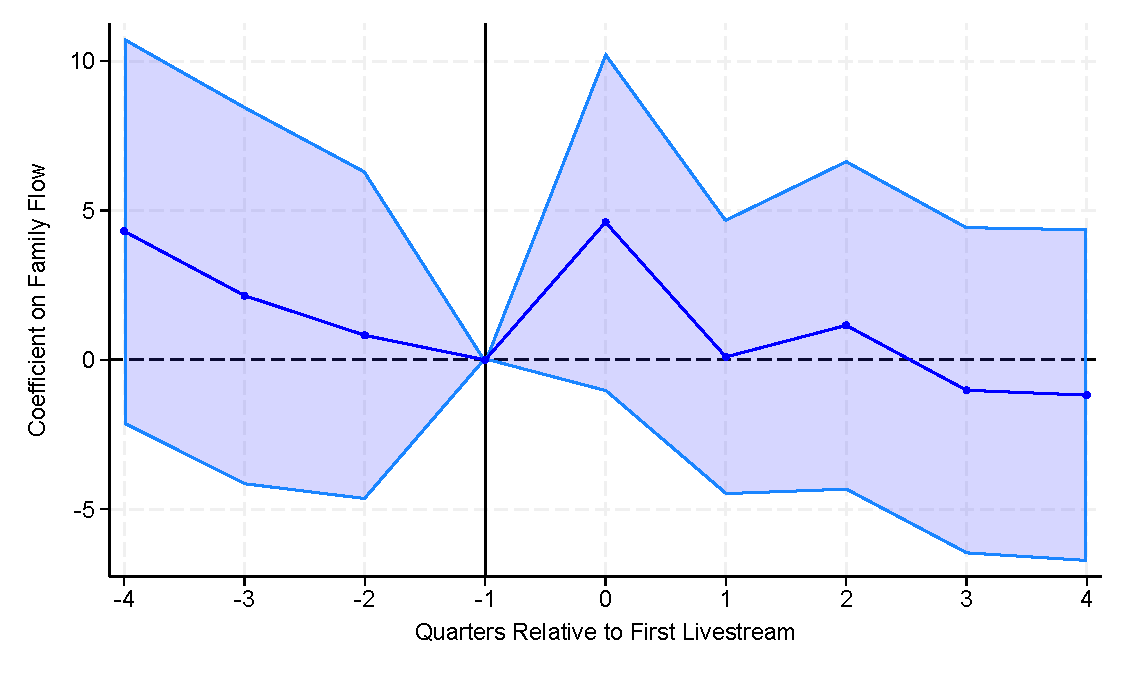
\includegraphics[width=0.70\textwidth]{pictures/family_twfe_event_study_plot.pdf}
\end{center}

\vspace{-0.2cm}
\muted{\small TWFE estimates of family flows around initial livestream adoption (quarter 0). Pre-event coefficients are flat (parallel trends hold). No sustained increase post-adoption.}

\end{frame}

% -----------------------------------------------------------------------

\begin{frame}{Fund-Level Decomposition: The Reallocation Mechanism}

\begin{center}
\resizebox{0.80\textwidth}{!}{%
\begin{tabular}{lccccc}
  \toprule
   & (1) & (2) & (3) & (4) & (5) \\
  \midrule
  Fund First Livestream
    & 14.13*** &            &          & 12.95*** &          \\
    & (1.89)   &            &          & (1.96)   &          \\[3pt]
  Fund Livestream
    &          &            & 14.87*** &          & 13.27*** \\
    &          &            & (1.85)   &          & (1.93)   \\[3pt]
  Family Livestream (Oth)
    &          &            &          & $-$1.49** & $-$1.94** \\
    &          &            &          & (0.70)   & (0.88)   \\[3pt]
  \midrule
  Controls & No & No & No & No & Yes \\
  \bottomrule
  \multicolumn{6}{l}{\muted{\small Fund FE, quarter FE. SE clustered at family. ***, ** = 1\%, 5\%.}}
\end{tabular}}
\end{center}

\vspace{0.1cm}
\begin{columns}[T]
\begin{column}{0.48\textwidth}
\begin{block}{Featured funds}
  Gain \hl{+13 to +15 pp} in quarterly flows ---
  $\approx$ one-third of within-fund flow SD.
\end{block}
\end{column}
\begin{column}{0.48\textwidth}
\begin{alertblock}{Non-featured siblings}
  Lose \hlg{$-2$ pp} --- opposing sign confirms
  within-family cannibalization.
\end{alertblock}
\end{column}
\end{columns}

\end{frame}

% -----------------------------------------------------------------------

\begin{frame}{Robustness: Family $\times$ Quarter Fixed Effects}

\textbf{Replace fund + quarter FE with family $\times$ quarter FE:}
\begin{itemize}
  \item Absorbs \emph{all} time-varying family characteristics:
  aggregate family flow, performance, market conditions
  \item Since family aggregate flow = 0 (previous results),
  this specification mechanically forces the coefficient to equal
  the \hl{full reallocation magnitude}
\end{itemize}

\vspace{0.25cm}
\begin{center}
\begin{tabular}{lccc}
  \toprule
   & Fund + Quarter FE & Family$\times$Quarter FE \\
  \midrule
  Fund Livestream & 14.87*** & 17.59*** \\
   & (1.85) & (2.25) \\
  \bottomrule
  \multicolumn{3}{l}{\muted{\small SE clustered at family level.}}
\end{tabular}
\end{center}

\vspace{0.25cm}
\begin{block}{Interpretation}
  The \hl{+17.6 pp} represents dollar-for-dollar reallocation: every dollar
  flowing into featured funds is offset by an equal dollar flowing out of
  non-featured siblings within the same family.
\end{block}

\end{frame}

% -----------------------------------------------------------------------

\begin{frame}{Performance of Featured vs.\ Non-Featured Funds}

\begin{center}
  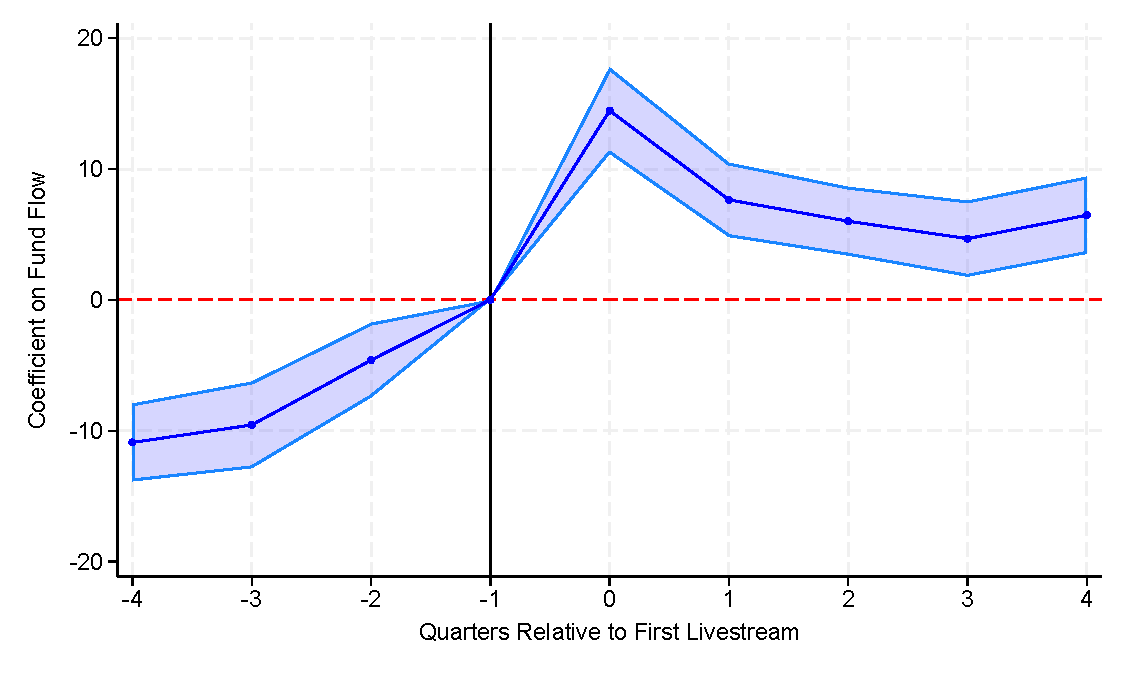
\includegraphics[width=0.70\textwidth]{pictures/fund_twfe_event_study_plot.pdf}
\end{center}

\vspace{-0.2cm}
\muted{\small Monthly raw returns of featured funds (blue) vs.\ non-featured siblings relative to the livestream event month. Fund and month fixed effects. Shaded bands: 95\% CI.}

\end{frame}

% -----------------------------------------------------------------------

\begin{frame}{Interpretation: Families as Open Market Operators}

\textbf{Before the livestream:}
\begin{itemize}
  \item Featured funds \hl{significantly outperform} non-featured siblings
  in months leading up to the event
  \item Non-featured funds underperform $\;\Rightarrow\;$ they are
  \textit{overcapitalized} relative to their skill (Berk \& Green, 2004)
\end{itemize}

\medskip
\textbf{After the livestream:}
\begin{itemize}
  \item Capital inflows erode featured funds' outperformance
  \item Capital outflows improve non-featured funds' performance
  \item Performance gap \hl{compresses} --- consistent with flow-performance
  equilibrium convergence
\end{itemize}

\vspace{0.2cm}
\begin{block}{Mechanism (Berk, 2017)}
  Families have \hl{superior information} about which funds are
  undercapitalized. Livestreaming steers existing investors
  from overcapitalized to undercapitalized funds.
  \textbf{Benefit:} retains investors who might otherwise search outside the family.
\end{block}

\end{frame}

% -----------------------------------------------------------------------

\begin{frame}{Fee Structure and Revenue: Also Zero}

\begin{columns}[T]
\begin{column}{0.52\textwidth}
\textbf{Could livestreaming shift flows toward higher-fee products?}

\medskip
\begin{itemize}
  \item \textbf{Management fees} (majority of revenue):\\
  \hl{no response} across all specifications and horizons
  \item \textbf{Service fees}: modest temporary increase
  of a few basis points, then reverts
  \item \textbf{Loads}: slight subsequent reduction
  \item Net effect: no systematic shift in family's fee structure
\end{itemize}

\medskip
\textbf{Flow-induced revenue} (fee $\times$ flow effects combined):
\begin{itemize}
  \item Statistically and economically insignificant
  across all specifications and horizons
\end{itemize}
\end{column}
\begin{column}{0.46\textwidth}
\begin{alertblock}{Bottom line}
  Families extract \hl{no additional revenue} from livestreaming.

  \medskip
  The zero-sum capital reallocation does not improve profitability.

  \medskip
  So why livestream at all?
\end{alertblock}

\vspace{0.2cm}
\begin{block}{Two answers}
  \begin{enumerate}
    \item Intra-family: optimize fund sizing (open market operation)
    \item Inter-family: defend market share from rivals
  \end{enumerate}
\end{block}
\end{column}
\end{columns}

\end{frame}

% -----------------------------------------------------------------------

\begin{frame}{Communication Strategies: What Attracts Outside Capital?}

\begin{columns}[T]
\begin{column}{0.52\textwidth}
\textbf{Approach:}
\begin{itemize}
  \item Define \textit{abnormal flows} = residuals from family
  flow regression on livestream intensity + controls
  \item Split into High (top 5\%) vs.\ Low (bottom 5\%)
  within each quarterly cross-section
  \item Sample 5 transcripts per family $\Rightarrow$ \hl{795 transcripts}
\end{itemize}

\medskip
\textbf{LLM scoring (Qwen-2.5-32B):}
\begin{itemize}
  \item \hl{16 dimensions}: sentiment, emotional intensity,
  sales pressure, past performance, social proof,
  educational content, risk transparency, \ldots
  \item Each scored 1--10 using a \textit{fixed rubric ex ante}
  \item Segment-level (10k chars), averaged to transcript
\end{itemize}
\end{column}
\begin{column}{0.46\textwidth}
\textbf{Results: only 2 of 16 dimensions differ}

\vspace{0.1cm}
\resizebox{\columnwidth}{!}{%
\begin{tabular}{lcc}
  \toprule
  Dimension & Diff. & $p$ \\
  \midrule
  \hl{Past Performance Focus} & \hl{$+$0.28} & \hl{.02} \\
  \hl{Social Proof Reliance}  & \hl{$+$0.23} & \hl{.04} \\
  \midrule
  Sentiment Positivity & $+$0.08 & .51 \\
  Emotional Intensity  & $-$0.05 & .68 \\
  Sales Pressure       & $+$0.11 & .39 \\
  Educational Content  & $+$0.03 & .82 \\
  \multicolumn{3}{l}{\muted{10 further dims: all insignificant}} \\
  \bottomrule
\end{tabular}}

\vspace{0.1cm}
{\small Investors respond to \textbf{verifiable ``hard'' information} ---
past returns and third-party validation --- not emotional appeals.}
\end{column}
\end{columns}

\end{frame}

% -----------------------------------------------------------------------

\begin{frame}{Competitive Equilibrium: The Defensive Motive}

\begin{columns}[T]
\begin{column}{0.52\textwidth}
\textbf{Within families (own vs.\ sibling effects):}
\begin{itemize}
  \item Own-fund livestreaming: \good{$+$7.2 pp} flows
  \item Sibling livestreaming: \bad{$-$4.9 pp} flows
  \item Net family effect: $\approx 0$
\end{itemize}

\vspace{0.2cm}
\textbf{Across families (market competition):}
\begin{itemize}
  \item When rivals increase livestreaming by 1 SD, non-livestreamers
  lose \hl{$\approx 27$ pp} in flows
  \item Market share in livestreaming activity strongly
  predicts fund-level flows ($+$620 pp per unit share)
\end{itemize}

\vspace{0.2cm}
\textbf{Implication:}\\
Families that stop livestreaming while rivals continue
face \emph{immediate} market share losses.
\end{column}
\begin{column}{0.46\textwidth}
\begin{block}{Prisoner's dilemma}
  Families must livestream \textbf{not to attract new investors}
  but to \hl{defend existing assets} from more actively
  marketed alternatives.

  \medskip
  Unilateral exit $\Rightarrow$ flow losses.\\
  Mutual participation $\Rightarrow$ zero net gain.

  \medskip
  Industry is trapped in a wasteful promotional arms race
  (Roussanov, Russ \& Wei, 2021).
\end{block}
\end{column}
\end{columns}

\end{frame}

% =============================================================================
\section{Conclusion}
% =============================================================================

\begin{frame}{Summary}

\begin{enumerate}\addtolength{\itemsep}{0.2cm}

  \item[\hlg{(1)}] \textbf{Zero-sum at the family level.}
  Livestreaming generates large fund-level inflows (\hl{+14 pp}) but
  zero family-level flow or revenue change.
  Featured funds gain at the direct expense of non-featured siblings.

  \item[\hlg{(2)}] \textbf{Intra-family capital optimization.}
  Families feature recently outperforming (undercapitalized) funds.
  Post-event performance converges --- consistent with Berk-Green
  rational learning. Livestreaming functions as an internal open
  market operation.

  \item[\hlg{(3)}] \textbf{Defensive arms race.}
  Families livestream to defend market share, not to expand it.
  Market-wide competition creates a prisoner's dilemma.

  \item[\hlg{(4)}] \textbf{Hard information wins.}
  Families that do attract outside capital emphasize past performance
  and social proof --- not emotional appeals or engagement style.

\end{enumerate}

\end{frame}

% -----------------------------------------------------------------------

\begin{frame}{Broader Implications}

\begin{wideitemize}

  \item \textbf{For the mutual fund literature:}\\
  Fund-level marketing effects do not imply family-level growth.
  Flow-performance sensitivities and marketing effectiveness must
  be evaluated at the family level.

  \item \textbf{For investor welfare:}\\
  Livestreaming facilitates within-family learning and capital
  allocation --- a genuine benefit. But aggregate marketing may
  be socially excessive: the industry is in a promotional arms race
  with no net new capital formation.

  \item \textbf{For policy:}\\
  AMAC's 2021 guidance (investor education, compliance controls)
  is well-targeted. Our evidence suggests the informative role of
  livestreaming (hard-info channel) coexists with a defensive
  market-share motive.

\end{wideitemize}

\bigskip
\begin{center}
  {\large \textcolor{myblue}{Thank you. Questions welcome.}}
\end{center}

\end{frame}

% =============================================================================
% Appendix
% =============================================================================
\appendix

\begin{frame}[shrink=5]{Appendix: Full Family-Level Flow Regressions}

\resizebox{\textwidth}{!}{%
\begin{tabular}{lcccccccc}
\toprule
 & (1) & (2) & (3) & (4) & (5) & (6) & (7) & (8) \\
\midrule
Family First Livestream & 3.77 & & & & & & & \\
 & (5.12) & & & & & & & \\[2pt]
Family Post Livestream & & $-$0.66 & & & & & & \\
 & & (2.34) & & & & & & \\[2pt]
Family Livestream & & & 0.90 & & & & 1.07 & \\
 & & & (2.17) & & & & (2.19) & \\[2pt]
Family Market Share & & & & $-$15.67 & & & & \\
 & & & & (18.43) & & & & \\[2pt]
Market Livestream (Oth) & & & & & $-$0.90 & & & \\
 & & & & & (1.65) & & & \\[2pt]
Family Livestream Count & & & & & & $-$0.09 & & 0.01 \\
 & & & & & & (0.50) & & (0.50) \\[2pt]
Market-Family Count & & & & & & & 24.55 & 14.52 \\
 & & & & & & & (20.33) & (18.47) \\[2pt]
\midrule
Family FE    & Y & Y & Y & Y & Y & Y & Y & Y \\
Quarter FE   & Y & Y & Y & Y & Y & Y & Y & Y \\
Controls     & Y & Y & Y & Y & Y & Y & Y & Y \\
\bottomrule
\multicolumn{9}{l}{\muted{\small SE clustered at family level. None significant.}}
\end{tabular}}

\end{frame}

% -----------------------------------------------------------------------

\begin{frame}{Appendix: Fund-Level Decomposition (Full)}

\begin{center}
\resizebox{0.82\textwidth}{!}{%
\begin{tabular}{lccccc}
\toprule
 & (1) & (2) & (3) & (4) & (5) \\
\midrule
Fund First Livestream
  & 14.13*** &          &          & 12.95*** &          \\
  & (1.89)   &          &          & (1.96)   &          \\[3pt]
Fund Post Livestream
  &          & 14.64*** &          &          &          \\
  &          & (2.01)   &          &          &          \\[3pt]
Fund Livestream
  &          &          & 14.87*** &          & 13.27*** \\
  &          &          & (1.85)   &          & (1.93)   \\[3pt]
Family Livestream (Oth)
  &          &          &          & $-$1.49** & $-$1.94** \\
  &          &          &          & (0.70)   & (0.88)   \\[3pt]
\midrule
Fund FE     & Y & Y & Y & Y & Y \\
Quarter FE  & Y & Y & Y & Y & Y \\
Controls    & No & No & No & No & Yes \\
\bottomrule
\multicolumn{6}{l}{\muted{\small ***, **, * = 1\%, 5\%, 10\%. SE clustered at family level.}}
\end{tabular}}
\end{center}

\end{frame}

% -----------------------------------------------------------------------

\begin{frame}{Appendix: Share Class Analysis}

\textbf{Specification:} Fund-quarter FE absorb all fund-level variation.
\[
\text{ClassFlow}_{c,q} = \delta_{f(c),q}
  + \beta_1\,\text{ClassLivestream}_{c,q}
  + \mathbf{X}'_{c,q-1}\Gamma + \varepsilon_{c,q}
\]

\begin{center}
\begin{tabular}{lcc}
\toprule
 & (1) & (2) \\
\midrule
Class Livestream & 10.20*** & \\
 & (2.34) & \\[4pt]
Solo Livestreamer (non-feat.\ class) & & $-$9.82 \\
 & & (8.15) \\[4pt]
Has Sibling Livestreamer & & $-$19.91 \\
 & & (14.60) \\[4pt]
\bottomrule
\multicolumn{3}{l}{\muted{\small Fund$\times$quarter FE. SE clustered at family level.}}
\end{tabular}
\end{center}

\medskip
Featured classes gain \hl{+10 pp} vs.\ non-featured classes of the \emph{same fund}
in the same quarter. Reallocation operates at every level: family $\to$ fund $\to$ share class.

\end{frame}

% -----------------------------------------------------------------------

\begin{frame}{Appendix: Performance Event Study (Robustness)}

\begin{columns}[T]
\begin{column}{0.49\textwidth}
  \centering
  \textbf{TWFE}\\[4pt]
  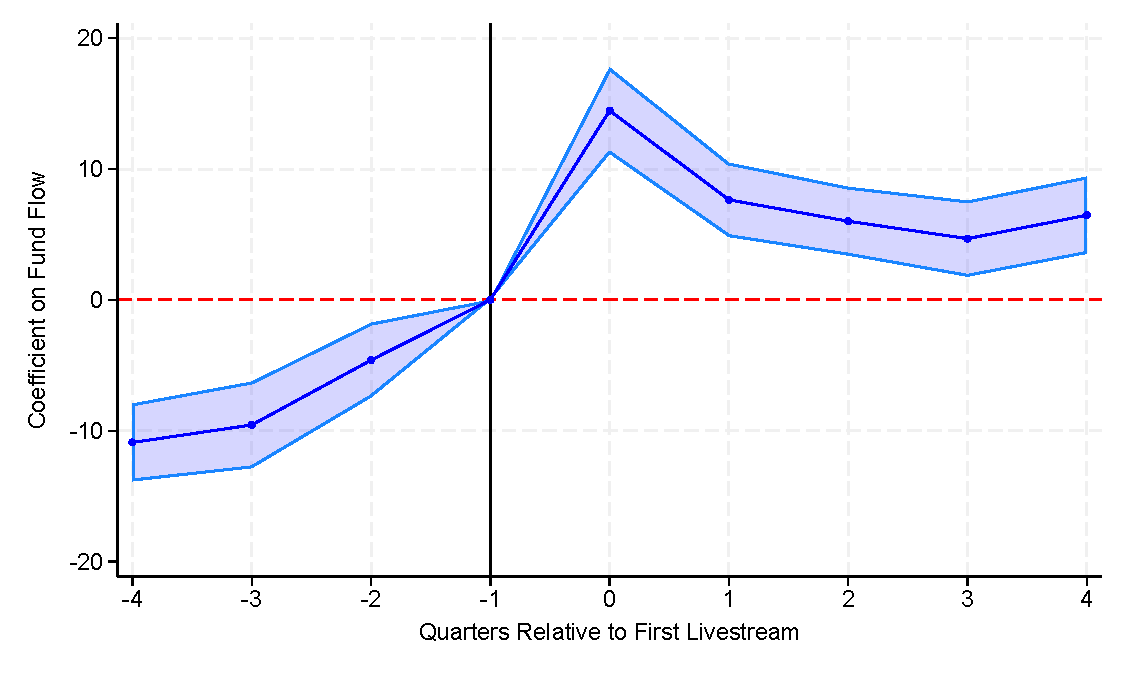
\includegraphics[width=\textwidth]{pictures/fund_twfe_event_study_plot.pdf}
\end{column}
\begin{column}{0.49\textwidth}
  \centering
  \textbf{Family$\times$Quarter FE}\\[4pt]
  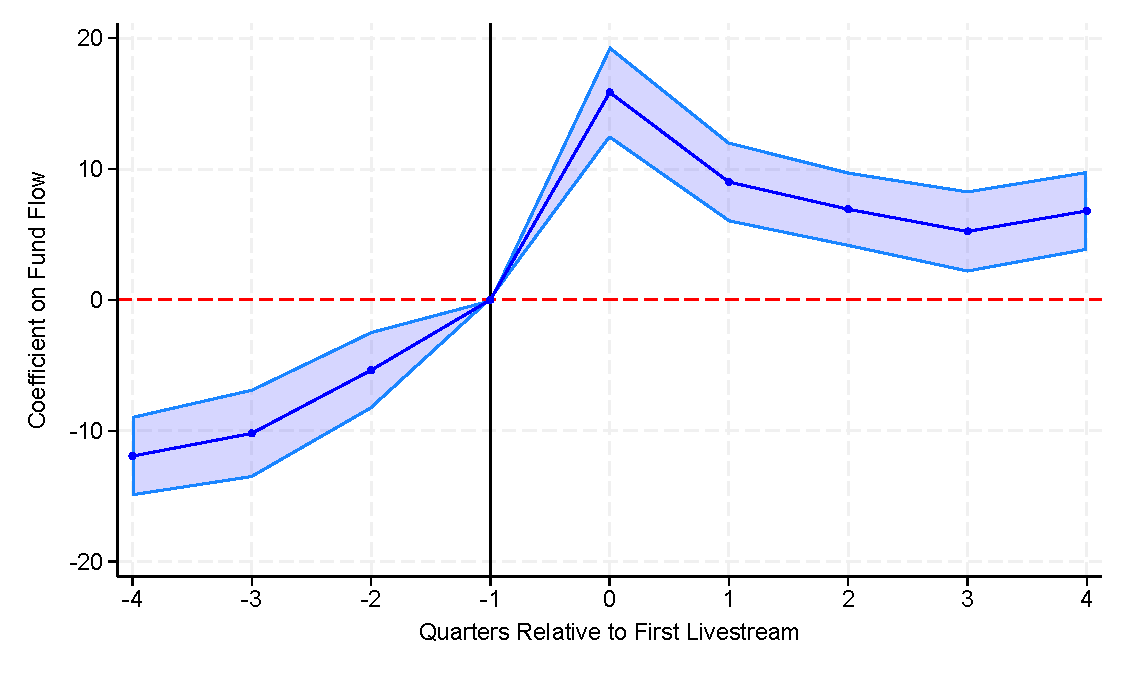
\includegraphics[width=\textwidth]{pictures/fund_hdfe_event_study_plot.pdf}
\end{column}
\end{columns}

\vspace{0.15cm}
\muted{\small Both specifications confirm pre-event outperformance of featured funds and post-event convergence. Robust to controlling for all time-varying family shocks.}

\end{frame}

% -----------------------------------------------------------------------

\begin{frame}{Appendix: LLM Scoring Dimensions (All 16)}

\begin{columns}[T]
\begin{column}{0.46\textwidth}
{\small
\begin{enumerate}
  \item Sentiment Positivity
  \item \hl{Past Performance Focus}$^*$
  \item \hl{Social Proof Reliance}$^*$
  \item Emotional Intensity
  \item Sales Pressure
  \item Educational Content
  \item Risk Transparency
  \item Community Building
\end{enumerate}}
\end{column}
\begin{column}{0.46\textwidth}
{\small
\begin{enumerate}
  \setcounter{enumi}{8}
  \item Urgency / FOMO
  \item Product Complexity Framing
  \item Presenter Credibility Signals
  \item Interactive Engagement
  \item Narrative / Storytelling
  \item Regulatory Compliance Emphasis
  \item Future Performance Claims
  \item Comparative Benchmarking
\end{enumerate}}
\end{column}
\end{columns}

\vspace{0.25cm}
{\small $^*$ Significantly different between high- and low-abnormal-flow families ($p < 0.05$).}

\vspace{0.15cm}
{\small \textbf{Scoring:} Qwen-2.5-32B; 10,000-char overlapping segments; 1--10 scale;
rubric fixed ex ante so measurement error is orthogonal to the strategies under study.}

\end{frame}

\end{document}
